% !TEX TS-program = lualatex
\documentclass[titlepage]{article}
\usepackage[a5paper,margin=0.5in]{geometry}

%% Header
\usepackage{fancyhdr,lastpage}
\usepackage[mmddyyyy]{datetime}
\renewcommand{\dateseparator}{/}
\fancypagestyle{plain}{
    \fancyhf{} %Clear Everything.
    \lhead{ VisLang Final Report }
    \rhead{ Page \thepage\ of \pageref{LastPage} }
    \setlength{\headheight}{24pt}
    \setlength{\footskip}{24pt}
    \renewcommand{\headrulewidth}{1pt} %0pt for no rule, 2pt thicker etc...
    \renewcommand{\footrulewidth}{0pt}
}
\pagestyle{plain}
\usepackage{indentfirst}

%%% For referencing items below
% TODO: This doesn't quite look right
% TODO: Somehow the LastPage number is highlighted
\usepackage[hidelinks]{hyperref}
\hypersetup{
    colorlinks,
    linkcolor={red!50!black},
    citecolor={blue!50!black},
    urlcolor={blue!80!black}
}
% Needed to use \autoref with listings from minted
\providecommand*{\listingautorefname}{Listing}
% Command for referencing listings
\newcommand*{\listingref}[1]{\nameref*{#1} (\hyperref[{#1}]{\autoref*{#1}})}

%% Tables 
\usepackage{longtable}
\newcommand{\specialcell}[2][l]{%
      \begin{tabular}[#1]{@{}c@{}}#2\end{tabular}
}

%% Figures
\usepackage{wrapfig}

%% Items
\usepackage{enumitem}

%% Code Listings
\usepackage{minted}
\usepackage{listings}
\usepackage{color} % for colored solution
\usepackage{caption}

% This will allow us to use file names with
% underscores in below
\AtBeginDocument{
    \catcode`_=12
    \begingroup\lccode`~=`_
    \lowercase{\endgroup\let~}\sb
    \mathcode`_="8000
}
% TODO: _ works in \inputminted but gets displayed in #2 as `
% TODO: don't print file name in list of listings
% TODO: put title of listing above code, not below it
% Custom macro for code listings from files
% #1 - language e.g. ocaml
% #2 - filename e.g. ../src/vislang.ml
% #3 - label e.g. src/top
% #4 - description e.g. Top Level
% note: filename will be pretty printed as vislang/src/*
%       instead of ../src/*
\newcommand{\srccode}[4]{
\clearpage
    \inputminted[linenos,fontsize=\footnotesize]{#1}{#2}
    \captionof{listing}{\label{#3}#4 File: #2}
\pagebreak
}

% custom language for log files
\lstset{%
    basicstyle=\ttfamily\scriptsize,
    keywordstyle=\color{blue}\ttfamily,
    stringstyle=\color{red}\ttfamily,
    commentstyle=\color{green}\ttfamily
}

% Custom macro for printing log file
% #1 - log filename
\newcommand{\inputlog}[1]{
    \lstinputlisting[nolol=true,language={}]{#1}
    \pagebreak
}

%% Diagrams
\usepackage{tikz}
\usetikzlibrary{shapes,arrows}
\tikzset{
    block/.style = {draw, 
                    rectangle, 
                    minimum height=2em, 
                    minimum width=12em,
                    node distance=1.5cm
    }
}

% For title page
\title{VisLang: A Visual Language\\Final Report}
\author{Bryant Eisenbach (UNI: bje2113)}
\date{Date: \today}

\begin{document}
% This command creates a title page
\maketitle
\pagebreak

\tableofcontents
\pagebreak

\listoffigures
\pagebreak

\listoftables
\pagebreak

\listoflistings
\pagebreak

\section{Introduction}

VisLang is a block diagram language designed to allow fast and
easy prototyping of programs for embedded processors. The language is created
with a graphical editor in mind, and the core language is designed to be extensible
so that any graphical editor can add additional elements or attributes for graphical
display or other features.

\subsection{Key Language Features}

The language itself is based on the idea of blocks: small parts that can be grouped
together into ever larger blocks and re-used across different programs. VisLang has a
small group of fundamental (or atomic) blocks that will be understood by the VisLang
compiler. Other blocks will be constructed as groupings of these atomic blocks, and can
be referenced in other files. Libraries of useful function blocks can be constructed
from these atomic blocks containing common parts such as timers, latches, etc. The 
ability to include blocks from libraries and other programs is a standard feature of
the language.

The syntax of VisLang leverages standard XML, giving the language a well-formed and 
machine readable backbone. As noted previously, the point of leveraging XML is so that
3rd party programs can manipulate the file format in an easy way, and so that external
programs can add additional elements (e.g. visual information for display) and attributes
(e.g. location information) to the existing set of elements and attributes defined by
the language. Those additional tags not included in the list of recognized elements/
attributes will be ignored by the compiler as a valid program is only defined as a series
of well-connected blocks. All parts have a set of necessary attributes, and all connections
require the source to exist. This creates a natural flow to interpreting the language, such
that only functional errors should be raised by the compiler during compilation.

The VisLang Compiler will parse and check the specified input file and generate a viable
C source file that can be used in combination with other generated and manually created
C source files to combine into fully functional programs for embedded devices. Each
generated file contains code that is completely reusable as the generated code has standard
interfaces and does not rely on global definitions. Some manual coding will still be
necessary to link into different types of embedded devices, the point is to create good
intermediate code such that linking to I/O devices and dealing with the nuances of an
arbitrary embedded device can be minimized.

\pagebreak

% TODO
\section{Language Tutorial}

The first group of elements (INPUT, OUTPUT, CONSTANT, NAME) provide named
memory locations for use in the application. All of these elements have a
type attribute where the datatype of the name is specified. INPUT, OUTPUT,
and SIGNAL have a scope attribute, which defines whether the name is local
scope (block-wide), global scope (program wide), or device scope (only
Inputs and Outputs can be device scope). When device scope is chosen, an
IO address must be chosen to specify where to read or write the I/O data
to the interface with the target hardware. The CONSTANT element describes
a named constant, which is initialized to the value provided and will reside
in memory and read each pass during program execution. All of these
elements have a size attribute, which means they can refer to array quantities
as well. A structure can be used as a datatype.

The second group of elements (PROGRAM, BLOCK, CONNECTION) describes block
constructs. This is the basis of how the program works. The PROGRAM element
is a container for the entirety of the program. The PROGRAM element has a
name attribute which describes what the compiled program should be
called by the compiler. The BLOCK element is also a container, but used
throughout the program to encapsulate functionality or define helper parts
in referenced files. BLOCK has an optional reference property which describes
the location of a block in a file using the "/path/to/file.vs$\vert$path$\vert$to$\vert$block"
syntax, where the vertical bars describe the heirarchy required to discover
the referenced block. Any referenced block will have to have connections to 
all of the defined inputs in the referenced block. The outputs are not
required.

The CONNECTION element is how blocks and parts are connected
together. The "to" attribute describes where the connection is headed, and
cannot have a different CONNECTION element with a matching "to" attribute
name. The "from" attribute describes where the connection came from, and
does not have the same restriction. Connections can either be made to named
signals such as INPUTS, OUTPUTS, CONSTANTS, or SIGNAL, or they can be made
implicitly to blocks themselves using "block$\vert$input" or "block$\vert$output" syntax.

The third group is the atomic parts. The Language Reference Manual will go
into more detail here but all of these parts should form the bare minimum 
required by the base language to compose all other required functions from.
All of the atomic parts operate on specific types and have a specific defined
function present in the compiler. All of the blocks have one or more inputs
(except DT) and have exactly 1 output. All of the blocks are time invariant,
,e.g. given the same input they produce the same output, except the DT
and MEM blocks. The MEM block will store the value of something until the next
pass. The DT block outputs the delta time between each pass. Since all blocks
are simple and operate on a defined amount of inputs and outputs, they can be
used with arrays to define parallel operations, e.g. applying the OR gate
operation against two boolean arrays of the same size to produce a third boolean
array of that same size. Structures will not work as inputs to these parts.

All the logic gates besides the NOT gate (AND, OR, etc.) as well as the BITWISE,
SUMMER, and PROD elements are defined as having two or more inputs (BITWISE can
be one if a mask is set). The way this works in practice is that each successive
input increments the number after the word "input" e.g. "input1", "input2",
"input3", etc. when making connections to these parts.

The fourth group describes array and structure utilities. MUX creates arrays from
a group of inputs with the same type, and similarly DEMUX will deconstruct an
array into a group of outputs of the same type. Similar to the atomic gate parts,
these parts allow on the relevant inputs/outputs a variable amount of elements
to be specified using the input\# syntax on the connection elements. The size of
arrays will be static during compilation, and array size will be a quantity traced
between blocks to verify size matching between usages.

CONSTRUCT and DESCTRUCT create and decompose STRUCT elements respectively. The
way this works is that a STRUCT element is defined seperately, with member
attributes defining the name and type of each member of the struct. The CONSTRUCT
element will allow a set of inputs matching the type of each of the members of a
struct to create a new named quantity of that structure, and similarly DESTRUCT
deconstructs a structure into signals that match each of those members. The STRUCT
element can be defined or referenced through a file, allowing a seperate definition
file to be reused over a project. Additionally, a STRUCT can be created from or written
to an array of certain types, using the exact amount of memory required with buffer
space as necessary to represent it as a chunk of memory. This will allow message
definitions to be encoded or decoded to/from a hardware buffer. Lastly, an array
can be composed of struct elements, as long as all elements match that structure
definition.

The last group of elements is the array functions. These functions operate on
arrays per element of the array, and require a referenced function of a certain
number and type of inputs/outputs to translate the input array into the output.
MAP will apply the referenced function of a single input to a single output
(that may or may not matches the input's type). What is important is that the input
array's type and the type of the input to the function match, as well as the
same criteria for the output.

FILTER is similar to MAP in that it has a referenced function, however the output is
required to be a boolean conditional. What FILTER will do is use that conditional
output to filter the input array into an output array. Since there is a design
decision not to allow variable array sizes, FILTER requires a size attribute for
the output, and will not update the output if the size does not match what the
attribute requires. This can be useful for parsing a buffer of word-based definitions,
as we can filter the array of words to find a single UID that is a part of the word
definition and pass that as the output to a parsing function.

The REDUCE element is similar to MAP and FILTER in that it takes an array
argument and use the function reference, however this function will take each
element of the array and apply it to a function that takes two inputs: the first
being the same type as each array element, and the second matching the output type
of the function. REDUCE will start with the first element and the initial value
for the output and recursively run through each element of the array, feeding back
the output as the inital value input for the next iteration. When REDUCE has
exhausted all of the elements of the array, the final output of the function
is returned back as the output of the REDUCE element.

Most attributes for elements are defined with a string. In some cases, it may be 
preferable to use a literal definition for a value instead of creating a reference
or using a named quantity. Every datatype in VisLang has a way of creating a literal.
Examples of literals for all VisLang types are below:
\begin{longtable}[c]{ |c|c| } 
    \hline
    datatype & example literal(s) \\ 
    \hline\hline
    boolean & false, true \\
    single, double & 1.000, 1e-6, 100 \\
    integer & 100, 0x20, 2x1011, 8x671, -120 \\ 
    \hline
    address & 0x1A56, 0x10A8$\vert$14 \\
    arrays & $[1, 2, 3, 4]$ \\
    structures & \{1, \{2, 3\}\} \\
    \hline
\end{longtable}

Booleans can only be false or true. Floating point quantities (single, double) can
be a decimal quantity (with or without significant digits after the decimal point),
or specified using scientific notation e.g. 10e6. Floating point literals can be
specified with a negative sign as well e.g. -1.234e-6. Integer quantities (e.g.
uint8, uint16, uint32, uint64, int8, int16, int32, int64) can be specified as a
decimal quantity (cannot have a decimal point), or using hex (e.g. 0x1A), binary
(e.g.2x1010), or octal (e.g. 8x2462) representation. Only signed integers can have
a negative sign in front. Additionally, for address literals, specifying a bit of
and address can be done with the $\vert$ operator against a hex representation of
the address (e.g. 0x1235$\vert$7). Address literals can only be in hex. Array
literals are created with the bracket operators (e.g. $[true, true, false]$), and
structure literals can be created using the braces operator (e.g. \{0x10, \{1, false\}\}.

Any attribute that accepts a literal can also take a reference to a named value,
in a similar way that block references are defined (e.g. "/path/to/file.vs$\vert$path$\vert$to$\vert$value").

\subsection{Example Program}

The following program illustrates some of the major features of the language. The
program itself takes a Digital Input on the target device, reads it, and starts a
timer when the input is enabled. When the timer counts up to the target time, it
will set a Digital Output true and reset the timer, creating a fast-blinking light
with a period of 2 seconds.

\srccode{xml}{../example/timed-blinking-light.vl}{example:top}{Example Top Level}

As noted, the above file contained a reference to another part called timer defined
in timer.vs in the same directory. Any references must take place on a relative path
to that file, and that reference must contain the same number of inputs specified by
the target file inside the file referencing that part. The number of outputs need
not match, but any outputs specified in the file referencing that part must also
match what is available from the target file or an exception will be thrown. All
other unused outputs will be disregarded. The following file displays the target
file, complete with the relevant inputs and outputs as specified/required by the
previous file.

\srccode{xml}{../example/timer.vl}{exmaple:timer}{Example Referenced Block}

\pagebreak

Below is the list of standard elements supported by the language, and their attributes:
\begin{longtable}[c]{ |c|c|c|c| } 
    \hline
    element & input(s) & outputs & attributes [optional]  \\ 
    \hline\hline
    INPUT & none & provides 'name' & scope, size, name, type, [address] \\ 
    OUTPUT & provides 'name' & none & scope, size, name, type, [address] \\ 
    CONSTANT & none & provides 'name' & size, name, type, value \\ 
    SIGNAL & provides 'name' & provides 'name' & scope, size, name, type \\ 
    \hline
    PROGRAM & device inputs & device, global outputs & name \\ 
    BLOCK & as defined & as defined & name, [reference] \\ 
    CONNECTION & none & none & to, from \\
    \hline
    CAST & input & output & name, type \\
    MEM & current & stored & name, initial\_condition \\
    DT & none & dt & name \\
    NOT & input & output & name \\
    AND & input\# (\# $>$ 1) & output & name \\
    OR & input\# (\# $>$ 1) & output & name \\
    NOR & input\# (\# $>$ 1) & output & name \\
    NAND & input\# (\# $>$ 1) & output & name \\
    XOR & input\# (\# $>$ 1) & output & name \\
    BITWISE & input\# (\# $>$ 0) & output & name, operation, [mask] \\
    IF & control, true, false & output & name \\
    COMPARE & lhs, rhs  & output & name, operation \\
    SUM & input\# (\# $>$ 1) & output & name \\
    PROD & input\# (\# $>$ 1) & output & name \\
    GAIN & input & output & name, value \\
    INV & input & output & name \\
    \hline
    MUX & input\# (\# $>$ 1) & provides 'array' & name, type, [address] \\
    DEMUX & array & output\# (\# $>$ 1) & name, type, [address] \\
    STRUCT & none & provides 'struct' & name, member\# (\# $>$ 0) \\
    CONSTRUCT & by definition & provides 'name' & name, definition \\
    DESTRUCT & struct & by definition & name, definition \\
    \hline
    MAP & input (array) & output (array) & name, func (SISO block ref) \\
    FILTER & input (array) & output & name, size, func (SIBO block ref) \\
    REDUCE & input (array) & output & name, initial\_value, func (MISO block ref) \\
    \hline
    SIGGEN & none & output & name, type, reference \\
    SCOPE & input\# (\# $>$ 1) & none & name, reference \\
\end{longtable}

\pagebreak

\section{Project Plan}

Since I was working on this project alone, there was more autonomy in creating the
language. This actually led to be a bit of a problem as my initial ideas for what
I wanted to accomplish were unrealistic and I was more willing to slide on the schedule
I set for myself since there were no other group members to act in the project manager
role to keep things on schedule, nor were any group members available to ensure that
project goals were reasonable. Regardless, after an initial development period of over
a month a working front end was developed leveraging the XML specification available
online with the planned tags and attributes I had at the time. It was eventually decided
that adding my own namespace for XML tags would be necessary to reduce the processing
load in the scanner and parser section to work with other elements. This is right around
the time the XML Abstract Syntax Tree was fully developed and work started on the backend
of the compiler.
\par
At this point, there was little testing in existance since I was just attempting to parse
the example program, so testing had to be approached. It was decided I was going to
leverage to bash testing script from the MicroC example language provided in class, and
have additional python scripts be created leveraging the Ctypes module to test the
functionality of each test case. Once this was decided, the first MWE test case was
developed (the buffer test case) and more work was done to get that to pass. More
complicated test cases led to a decision to add a complete block parsing algorithm in
order to be able to produce a correctly formatted program for code generation. After
some development, this algorithm allowed more test cases to pass and work to continue
on integrating block group and referencing functionality. Once this was completed, the
initial draft of VisLang was considered feature complete, and several other planned
features were descoped due to time constraints on the project.

\subsection{Software Development Environment}

Development for the project took place entirely on an Asus Chromebook C720 using crouton
to enable a full linux environment. The tools used for this project are listed below:

\begin{itemize}
\item ubuntu 14.04.2 LTS (Operating system environment)
\item git 1.9.1 (source code, test, and documentation configuration management)
\item vim 7.4.52 (general purpose text editor)
\item ocaml 4.01.0 (including ocamlyacc and ocamllex)
\item gcc 4.8.2 (compiling generated code)
\item python 2.7.6 (scripting language for testing compiled C objects)
\end{itemize}

\subsection{Project Timeline}

\begin{itemize}
\item 2015-05-27  Decided on Simulink-like block language, using XML syntax
\item 2015-05-31  Created example program
\item 2015-06-12  Proposal Submitted
\item 2015-06-21  First draft of scanner
\item 2015-06-26  First draft of parser
\item 2015-06-30  Scanner working for all attributes and tags
\item 2015-07-04  LRM Submitted
\item 2015-07-08  Parser working for new ast
\item 2015-07-09  Added top level
\item 2015-07-10  Moved errors to their own module
\item 2015-07-14  XML ast working
\item 2015-07-17  Integrated blockification function
\item 2015-07-24  Removed interpreter
\item 2015-07-27  Simplified blockification process
\item 2015-07-28  Moved trace algorithm from blockify to it's own module
\item 2015-08-05  Working Code Generation for all atomic parts
\item 2015-08-12  Got blocks completely working end-to-end
\item 2015-08-12  Updated blockification for Reference part
\item 2015-08-13  Began working on paper
\item 2015-08-14  Submitted paper
\item 2015-08-15  Celebrated from Canada
\end{itemize}

\subsection{Project Log}
\inputlog{../git.log}

\pagebreak

\section{VisLang Compiler Architecture}

\begin{wrapfigure}[25]{r}[-1.2cm]{0.25\textwidth}
  \centering
  \begin{tikzpicture}[auto]
    \node [block]                   (source)  {Source File (XML)};
    \node [block,below of=source]   (xmltok)  {XML Tokens};
    \node [block,below of=xmltok]   (xmlobj)  {XML Object Tree};
    \node [block,below of=xmlobj]   (blkobj)  {Block Object Tree};
    \node [block,below of=blkobj]   (optblk)  {Optimized Block Tree};
    \node [block,below of=optblk]   (gencod)  {Auto-generated Code};

    \draw[->] (source) -- node{xscanner.mll}    (xmltok);
    \draw[->] (xmltok) -- node{xparser.mly}     (xmlobj);
    \draw[->] (xmlobj) -- node{blockify.ml}     (blkobj);
    \draw[->] (blkobj) -- node{blockparse.ml}   (optblk);
    \draw[->] (optblk) -- node{compile.ml}      (gencod);
  \end{tikzpicture}
  \caption{VLCC Architecture}
  \label{arch:vlcc}
\end{wrapfigure}

The architecture of VisLang has two distinct stages of operation from source file to
target file. The scanning and parsing stages of the front end essentially implement
read the XML elements of interest and skip through parsing any unrecognized tokens.
After a correctly formed XML Object Tree has been formed, the next step is to translate
that tree of XML Objects (an XML Object has a tag, a list of attributes and a list of
inner objects, if any) into a block tree where each block can verify and access the
necessary attributes it should have. Each object can also see the list of connections
assigned to it when it was parsed, which is important when verifying the program is
well-formed. That block tree is then taken and re-organized such that the inner objects
of a block are in Static Single Assignment form, e.g. each block can be computed using
the outputs of previous blocks in the list for that containing block.
\par
In the process of reorganizing the inner blocks, the Block Parse algorithm will also
perform the check that the inner blocks align (e.g. they call blocks that are properly
assigned, they match in datatype, etc.) and that only inner blocks which are used to
compute the output are in the calculation. Any blocks which do not align will raise an
error (datatype mismatch, incorrectly attributes for that object, etc.), any blocks
which reference other blocks in a circular fashion will raise an error (algebraic loop),
and any blocks that are not necessary to compute an output will be optimized away. The
end result is that the remaining optimized block tree is a suitable candidate to be
directly translated into generated code as that generated code will have the property
of minimal side-effects: all computations are computed either from inputs or derived
from inputs.

\pagebreak

\section{Test Plan}

The generated target code for \autoref{example:top} and \autoref{example:timer}
from the Tutorial are below:

\srccode{C}{../example/timed-blinking-light.c}{gen:top}{Generated Code for Top Level}
\srccode{C}{../example/timer.c}{gen:timer}{Generated Code for Referenced Block}

The output program, when compiled using gcc, will be able to process the inputs provided
by 'connecting' to that block and update it's outputs over time for every iteration of
the program in the main loop. For programs without MEM or DT blocks, the resulting code
has the property of being time-invariant, that is no matter how many times it is called
or whatever the duration between calls are, it will produce the exact same result every
time. The MEM element will remember a value between the last call and the current such
that the resulting program loses that time invariance, but this operation allows the
production of functionality such as states and transfer functions to be modeled using
VisLang. The DT element is used when the amount of time between calls is important,
but for a steady system this should never be an issue as it should stay relatively
constant. This means programs using DT may or may not be almost time invariant, but
that depends on the usage of the block.
\par
To automate testing of VisLang programs, a shell script (\autoref{test:script}) was
borrowed from the MicroC example language. The shell script looks at all of the files
in a directory and processes them into 1 of 3 testing groups: test, pass, fail. The pass
and fail testing groups simply looks to verify that the source file for such a test case
either pass compilation (pass cases) or fails compilation (fail). In this way, specific
compiler features that have to do with processing the input file (instead of the code
generated) can be checked without further complication. The 'test' cases first verify that
the source file can generate the target file, but additionally a functional check is
provided through associated *.in and *.out files that are run against the target file.
\par
The methodology for testing these cases involves additionally compiling the target files
as source files for gcc, and turning the resulting object file into a shared library that
can be interpreted through a testing script. The testing script is a python script that
is generated using the -d option of vlcc which takes the *.in file and runs a while loop
over each line of the file and produces what the output of the program would be for each
timestep. The timestep is purposely never updated to ensure that a repeatable test
environment exists. The output produced by the test script is then compared against the
associated *.out file to see if any differences exist. If the two files match, then the
test is determined to be passing.

\subsection{Test Case List}

The following is a list of the test cases used to verify the VisLang compiler produces
correct code:

\begin{longtable}[c]{ |r|p{6cm}| }
    \caption{Test Case Descriptions}
    \label{table:testcases}
    \hline
    Test Case                   & Description \\
    \hline
    \hline
    \listingref{test:failal}    & Shows that an algebraic loop is caught \\
    \hline
    \listingref{test:failbc}    & Shows that a badly specified connection is caught \\
    \hline
    \listingref{test:failma}    & Shows that a missing attributes in a block is caught\\
    \hline
    \listingref{test:failub}    & Shows that an unended block is caught \\
    \hline
    \listingref{test:passeb}    & Shows that an empty block compiles okay \\
    \hline
    \listingref{test:failceb}   & Shows that multiple empty blocks inside each other are okay\\
    \hline
    \listingref{test:passg}     & Shows that random XML and other input is okay between tags \\
    \hline
    \listingref{test:testb}     & Shows proper operation of buffer block (O = I)\\
    \hline
    \listingref{test:testbib}   & Shows that a block within a block works \\
    \hline
    \listingref{test:testm}     & Shows the memory block works okay \\
    \hline
    \listingref{test:testc}     & Shows all the comparision operations work \\
    \hline
    \listingref{test:testg}     & Shows all the logical gates work \\
    \hline
    \listingref{test:testmc}    & Shows all math blocks work okay \\
    \hline
    \listingref{test:tesths}    & Shows a reference block works okay \\
    \hline
    \listingref{test:testsrl}   & Shows that a complex block (SR Latch) works \\
    \hline
    \listingref{test:testt}     & Shows that example (Timer block) works \\
    \hline
\end{longtable}

\pagebreak

\section{Conclusion}

The VisLang compiler was moderately a success because it lays the groundwork for future
iterations of the program for use in a fully optimized environment as a replacement for
developing embedded programs using proprietary IDEs or programming languages that are
more difficult to understand. A variety of lessons where learned during the development
of the program that will be detailed below. As a result of several of the lessons learned,
suggestions for future development are also presented.

\subsection{Lessons Learned}

The original idea for VisLang was very ambitious: to make a general purpose embedded
computing language in a visual format that could be used to develop programs for
small embedded devices such as the Aruduino platform. Early on the in the project
it was realized that this is much to ambitious of a goal because that would mean 
essentially replicating the avr C libraries in a language that was not meant for it.
Instead, the scope of VisLang was first pared down such that VisLang instead generated
C code instead of assembly so that it would be easy to link with the already feature-
complete libraries that exist for the platform. Integration with the avr libraries
remains untested at this time, but it is easy to show how VisLang-generated code could
be easily integrated into while loop almost any embedded device utilizes to run code.
The thought is that the specialty code needed to interface with the device is only a
small portion of the overall code the user is interested in running, so such a tradeoff
would be acceptable.
\par
Another lesson that was learned a few weeks into development of VisLang was that testcase
driven development would be required to move forward at an acceptable pace. Originally,
the development philosophy was trying to implement all of the required features of the
language at once, but even trying to get the simplest program (a buffer block, which passes
input directly to output) was a difficult task and a philosophy change was needed. A test
case for the buffer block was written and the compiler was made to work appropiately with
that test case first before further test cases were developed and more functionality was
implemented to meet those new cases. The benefits of this approach primarily are that these
test cases are available for quick turnover later on to validate future changes to the code.
This happened several times where a change made to satisfy one test case ultimately did,
but broke several of the already completed test cases. Integrating test cases into
development was one of the biggest lessons learned at first.
\par
Finally, the last lesson that was learned was to complete more preliminary work before
creating a specification for a language. Knowing how much would be possible as well as
prototyping some of the features beforehand would have helped to write a much more sound
specification to begin with so that scope reduction and philosophy changes would be
minimized.

\subsection{Future Improvements}

Several pieces of VisLang's original specification were descoped for the initial version
of the compiler due to time constraints. Given future development time, most of these
features would be required for VisLang to reach it's full potential as a general purpose
prototyping and embedded controller language to match potential rivals such as Simulink
and Modelica.
\par
First off, a graphical interface for manipulating VisLang code would make development of
programs in the language much easier, since that was the original intended use-case.
Significant development would be necessary here, but thankfully true to the original
design goals development to VisLang and any GUI environment that might use the language
could happen mostly in parallel. Specific attention would need to be taken to overhaul
VisLang's front end to make it truly resilient to non-VisLang XML elements. As it stands
right now, VisLang supports ignoring additional attributes, but using attributes of the
same name can confuse the parser which will throw an error. Either an alternative way to
specify VisLang attributes would need to be attempted, the VL Compiler would need to be
hardened against those attributes by more clever design of the front end, or a better
methodology of specifying the XML would need to be investigated to satisfy this goal.
\par
Arrays and Structures would be essential to truly allowing the language to prosper in
all of its intended use cases. Originally, the Array features of VisLang would allow a
user to create and pass around Arrays to inputs, enabling Function Language elements such
as Filter, Reduce, and Map to be applied so duplicate functionality can be performed with
minimal coding. This is important to larger embedded devices because they typically have
redundant interfaces that require the exact same processing to each element. Additionally,
digital busses can be arrays of packet structures that need the exact same processing
where a language that operated on them in parallel would be able be more efficient in its
operation. Structures would be used in a similar way, enabling I/O messages to be stripped
apart and processed in a predictable way, or output messages to be created in a specified
manner.
\par
Of course, a block language like VisLang can always support more parts. The original
specification for VisLang included several parts that were deemed unnecessary for the
initial implementation of the compiler, so identifying and adding that functionality
would be an obvious next step for the language. Adding the ability to encapsulate or link
to arbitrary code would also be another possible design goal for VisLang as often it is
necessary to have a calculation drive some action that interfaces with the embedded
processor, such as servicing the watchdog timer or managing interrupts. This would be
important if VisLang were to be used on larger projects.

\pagebreak

\appendix

\section{VLCC Source Code}
\srccode{ocaml}{../src/vislang.ml}{src:top}{Top Level}
\srccode{ocaml}{../src/xscanner.mll}{src:scan}{XML Scanner}
\srccode{ocaml}{../src/xparser.mly}{src:parse}{XML Parser}
\srccode{ocaml}{../src/xst.ml}{src:xst}{XML Syntax Tree}
\srccode{ocaml}{../src/blockify.ml}{src:blockify}{XML Object to Block Object Converter}
\srccode{ocaml}{../src/blockparse.ml}{src:bparse}{Block Object Ordering and Optimization}
\srccode{ocaml}{../src/compile.ml}{src:compile}{Code Generation}
\srccode{ocaml}{../src/errors.ml}{src:errors}{VisLang Errors}

\section{VLCC Utilities}
\srccode{make}{../src/Makefile}{util:make}{Automated Build Script}
\srccode{bash}{../test/run_tests.sh}{test:script}{Automated Testing Script}

\section{VLCC Test Cases}
\srccode{xml}{../test/fail-algebraic_loop.vl}
    {test:failal}{Algebraic Loop Failure Case}
\srccode{xml}{../test/fail-bad_connection.vl}
    {test:failbc}{Bad Connection Failure Case}
\srccode{xml}{../test/fail-missing_attribute.vl}
    {test:failma}{Missing Attribute Failure Case}
\srccode{xml}{../test/fail-unended_block.vl}
    {test:failub}{Unended Block Failure Case}
\srccode{xml}{../test/pass-cascaded_empty_blocks.vl}
    {test:failceb}{Cascaded Empty Blocks Completion Case}
\srccode{xml}{../test/pass-empty_block.vl}
    {test:passeb}{Empty Block Completion Case}
\srccode{xml}{../test/pass-gibberish.vl}
    {test:passg}{XML Tolerance Case}
\srccode{xml}{../test/test-buffer.vl}
    {test:testb}{Buffer Value Test Case}
\srccode{xml}{../test/test-buffer_in_buffer.vl}
    {test:testbib}{Buffer in Buffer Value Test Case}
\srccode{xml}{../test/test-compare.vl}
    {test:testc}{Comparision Operation Test Case}
\srccode{xml}{../test/test-gates.vl}
    {test:testg}{Logical Gate Test Case}
\srccode{xml}{../test/test-hysteresis_sw.vl}
    {test:tesths}{Reference Block Test Case}
\srccode{xml}{../test/test-math_constant.vl}
    {test:testmc}{Math Operations Test Case}
\srccode{xml}{../test/test-memory.vl}
    {test:testm}{Memory Block Test Case}
\srccode{xml}{../test/test-set_reset_latch.vl}
    {test:testsrl}{SR Latch Complexity Test Case}
\srccode{xml}{../test/test-timer.vl}
    {test:testt}{Timer Complexity Test Case}


\end{document}
